\begin{frame}{Przyk�ad}

	\begin{center}
	
		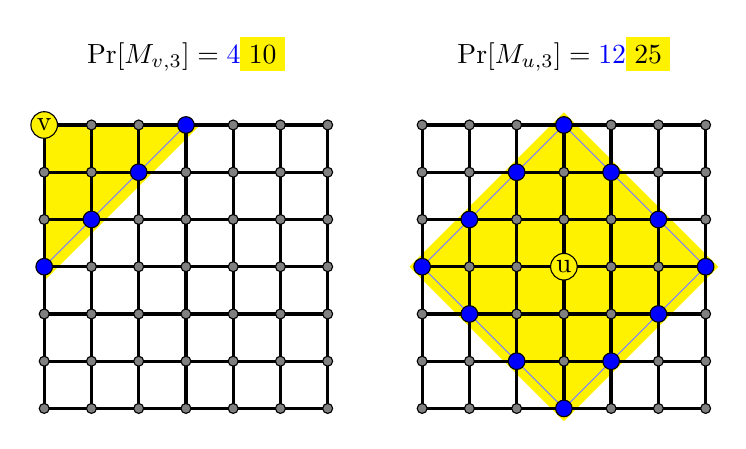
\begin{tikzpicture}[scale=0.6]
		\node at ( 3,7.5)  () {
		 $\Pr[M_{v,3}]=\slfrac{\textcolor{blue}{4}}{\colorbox{yellow}{10}}$
		};
		\node at ( 11,7.5)  (){ 
		 $\Pr[M_{u,3}]=\slfrac{\textcolor{blue}{12}}{\colorbox{yellow}{25}}$                   
		};
		
		\fill[yellow!100] (0,6) node {}  -- (0,2.7) node {}  -- (3.3,6) node {} ;
		\filldraw[rotate around={45:(11,3)}] [yellow!100] (8.7,0.7) rectangle (13.3,5.3);
		\draw [very thick] (0,0) grid (6,6);
		\foreach \i in {0,1,...,6}
		\foreach \j in {0,1,...,6}
		\filldraw[draw=black!100,fill=black!50](\i,\j) circle (3pt);
		
		\draw [very thick] (8,0) grid (14,6);
		\foreach \i in {8,9,...,14}
		\foreach \j in {0,1,...,6}
		\filldraw[draw=black!100,fill=black!50](\i,\j) circle (3pt);
		
		
		\filldraw[draw=black!100,fill=yellow!100](0,6) circle (8pt);
		\node at ( 0,6)   () {v};
		\filldraw[draw=black!100,fill=yellow!100](11,3) circle (8pt);
		\node at ( 11,3)   () {u};
		
		\draw [blue!50] (0,3) -- (6-3,6);
		\filldraw[draw=black!100,fill=blue](0,3) circle (5pt);
		\filldraw[draw=black!100,fill=blue](1,4) circle (5pt);
		\filldraw[draw=black!100,fill=blue](2,5) circle (5pt);
		\filldraw[draw=black!100,fill=blue](3,6) circle (5pt);
		
		\draw [blue!50] (11,6)--(14,3)--(11,0)--(8,3)--cycle;
		\filldraw[draw=black!100,fill=blue](8,3) circle (5pt);
		\filldraw[draw=black!100,fill=blue](14,3) circle (5pt);
		\filldraw[draw=black!100,fill=blue](9,4) circle (5pt);
		\filldraw[draw=black!100,fill=blue](13,4) circle (5pt);
		\filldraw[draw=black!100,fill=blue](10,5) circle (5pt);
		\filldraw[draw=black!100,fill=blue](12,5) circle (5pt);
		\filldraw[draw=black!100,fill=blue](11,6) circle (5pt);
		\filldraw[draw=black!100,fill=blue](9,2) circle (5pt);
		\filldraw[draw=black!100,fill=blue](13,2) circle (5pt);
		\filldraw[draw=black!100,fill=blue](10,1) circle (5pt);
		\filldraw[draw=black!100,fill=blue](12,1) circle (5pt);
		\filldraw[draw=black!100,fill=blue](11,0) circle (5pt);
		
		\end{tikzpicture}
	\end{center}

\end{frame}


